% =====================================================================
% Problems A-D. Figures: replace the example-image-* placeholders with
% your exported figures (see the % TODO comments). Code links: fill in
% the blue placeholders. Everything else reflects the executed runs.
% =====================================================================

%%%%%%%%%%%%%%%%%%%%%%
\chapter{Problem A}
\label{ch:problem_A}
%
\section{Problem Description}
A rod of unit length is loaded by a constant body force and clamped at both
ends. Its static response is governed by
\begin{equation}
    -\frac{d}{dx}\Big(k(x)\,\frac{du}{dx}\Big) = f, \qquad x \in (0,L),
    \qquad u(0) = u(L) = 0,
    \label{eq:A_pde}
\end{equation}
with $f = 9.81$ and $L = 1$. The Young's modulus $k(x) > 0$ is unknown. What
is available instead is a set of $N_{obs} = 500$ displacement measurements
$u_{obs}$ at randomly placed sensor positions $x_{obs}$, contaminated by
roughly $5\%$ noise. The task is an inverse problem: reconstruct the
coefficient $k(x)$ from the noisy observations of the state $u(x)$. The
quality of the reconstruction is measured by the relative $L^2$ error
against a reference given on a fine grid of $10001$ points, which is used
for evaluation only.
%
\section{Methodology}
%
\subsubsection{The method selection}
We solve the inverse problem with a physics-informed neural network (PINN)
in the formulation of \cite{raissi2019pinn}, using two separate networks:
$u_\theta(x)$ for the displacement and $k_\phi(x)$ for the modulus. The
choice is motivated by three properties of the problem. First, the
observations are scattered and noisy, so a mesh-based identification would
require an explicit smoothing step; a neural network fitted by least
squares performs this smoothing implicitly. Second, the PDE residual
couples $u$ and $k$ through derivatives, and automatic differentiation
supplies exact derivatives of the smooth surrogate $u_\theta$ (the noisy
data) itself is never differentiated. Third, prior knowledge is easy to
build into the ansatz: the clamped boundary conditions and the positivity
of the modulus are enforced exactly by output transforms,
\begin{equation}
    u_\theta(x) = x\,(L-x)\,\mathcal{N}_u(x;\theta), \qquad
    k_\phi(x) = \mathrm{softplus}\big(\mathcal{N}_k(x;\phi)\big),
\end{equation}
where $\mathcal{N}_u$ and $\mathcal{N}_k$ are fully connected networks. The
positivity constraint is not cosmetic. Integrating \eqref{eq:A_pde} once
gives the flux relation $k\,u' = -f x + C$; the constant $C$ is fixed only
by requiring that $k$ remains finite and positive at the interior point
where $u'$ vanishes, so the softplus transform is what makes the problem
identifiable.

An important practical finding: minimizing the data loss and the residual
loss jointly from a random initialization consistently converged to a poor
local minimum in which $k_\phi$ stayed nearly constant (its error settled
at the level of the best constant approximation of the true, oscillatory
modulus). We therefore train in two stages. Stage one fits $u_\theta$ to
the observations alone until the data loss reaches the noise floor. Stage
two freezes $u_\theta$ and recovers $k_\phi$ from the PDE residual,
regularized by a Tikhonov-type smoothness penalty, which is standard
practice for noisy coefficient identification.
%
\subsubsection{The loss function}
Stage one minimizes the mean-squared data misfit
\begin{equation}
    \mathcal{L}_{data}(\theta)
    = \frac{1}{N_{obs}}\sum_{i=1}^{N_{obs}}
      \big(u_\theta(x_{obs}^{(i)}) - u_{obs}^{(i)}\big)^2 .
\end{equation}
Stage two minimizes, with $u_\theta$ frozen,
\begin{equation}
    \mathcal{L}_{pde}(\phi)
    = \frac{1}{N_c}\sum_{j=1}^{N_c}
      \Big(\tfrac{1}{f}\big[-\big(k_\phi\,u_\theta'\big)'(x_c^{(j)}) - f\big]\Big)^2
      + w_{reg}\,\frac{1}{N_c}\sum_{j=1}^{N_c}\big(k_\phi'(x_c^{(j)})\big)^2 ,
\end{equation}
where all derivatives are computed by automatic differentiation. The
$N_c = 2000$ collocation points are redrawn uniformly in $(0,L)$ at every
epoch, which acts like an unlimited training set. Dividing the residual by
$f$ makes both loss terms of order one, so no weight is needed between the
data and residual terms; the only tuned weight is the smoothness penalty,
$w_{reg} = 10^{-4}$ (the recovered $k$ was insensitive to this value over
roughly two orders of magnitude).
%
\subsubsection{The network structure}
Both networks share the architecture in Table~\ref{tab:problem_A_net};
together they have $10502$ trainable parameters.
%
\begin{table}[htbp]
\centering
\caption{Network architecture used for both $\mathcal{N}_u$ and $\mathcal{N}_k$ (Problem A).}
\label{tab:problem_A_net}
\begin{tabular}{llll}
\hline
\textbf{Layer} & \textbf{Size / Neurons} & \textbf{Activation} & \textbf{Notes} \\
\hline
Input          & 1   & --    & coordinate $x$ \\
Hidden 1--3    & 50  & tanh  & fully connected \\
Output         & 1   & --    & linear; then $x(L-x)\cdot(\,\cdot\,)$ for $u$, softplus for $k$ \\
\hline
\end{tabular}
\end{table}
%
\subsubsection{The code link}
{https://github.com/omkulkarni01/PDE_Om_Anant_Kulkarni/blob/main/Problem_A.ipynb}
%
\section{Numerical Experiments}
%
\subsubsection{Experiment Setups}
%
\begin{table}[htbp]
\centering
\caption{Numerical setup for training (Problem A).}
\label{tab:problem_A_setup}
\begin{tabular}{ll}
\hline
\textbf{Parameter} & \textbf{Value} \\
\hline
Optimizer                  & Adam \\
Learning rate (initial)    & $1\times10^{-3}$ (both stages) \\
Batch size                 & full batch (500 sensors; 2000 collocation points) \\
Number of epochs           & 8000 (stage 1) $+$ 8000 (stage 2) \\
Learning rate scheduler    & StepLR, $\times 0.5$ every 2000 / 2500 epochs \\
Loss weights               & $w_{data}=1$, $w_{pde}=1$, $w_{reg}=10^{-4}$ \\
Hardware                   & NVIDIA GeForce RTX 4050 Laptop GPU \\
Precision                  & Float32 \\
Random seed                & 1234 \\
\hline
\end{tabular}
\end{table}
%
Tricks that improved the results: the hard boundary constraint (removes one
loss term entirely), the softplus positivity transform (identifiability,
see above), normalization of the residual by $f$, resampling of the
collocation points at every epoch, the two-stage curriculum, and
checkpointing of the model at the lowest training loss of each stage. The
test set was used exclusively to record the error curve, never for model
selection.
%
\subsubsection{Numerical Results}
Training took $121.8$~s in total. Stage one drives the data loss to
$8.66\times10^{-4}$, which equals the empirical variance of the observation
noise ,the network fits the signal and averages the noise out. The final
relative $L^2$ errors are $1.18\times10^{-1}$ for $k$ and
$5.07\times10^{-3}$ for $u$. The pointwise error of $k$ is strongly
concentrated around $x = 0.5$. This has a structural reason: there the flux
$k\,u'$ degenerates because $u'$ changes sign, and the coefficient is
determined only through the second derivative of the noisy state, which is
the quantity most affected by the $5\%$ noise. Away from this degenerate
region the modulus is recovered to within a few percent.
%
\begin{figure}[ht]
    \centering
    \begin{subfigure}[b]{0.5\textwidth}
        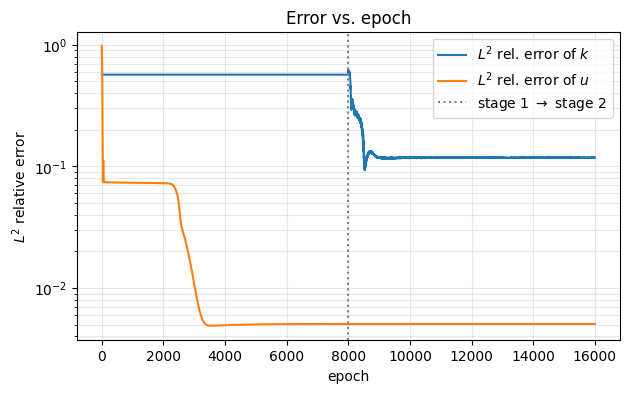
\includegraphics[width=\textwidth]{figures/ProblemA_L2vsepoch.png} % TODO: error-vs-epoch curve
        \caption{Relative $L^2$ error vs.\ epoch ($k$ and $u$).}
    \end{subfigure}
    %
    \begin{subfigure}[b]{0.5\textwidth}
        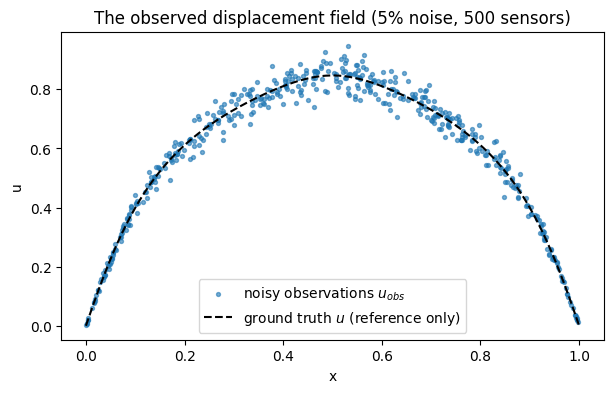
\includegraphics[width=\textwidth]{figures/ProblemA_noisy_obs.png} % TODO: observations + fitted u
        \caption{Noisy observations and fitted displacement.}
    \end{subfigure}
    \caption{Problem A: training history and data fit.}
    \label{fig:problem_A_1}
\end{figure}
%
//
\paragraph{Interpretation and possible improvements:}
The two error levels are direct consequences of how the chosen model
processes the data. The PINN recovers $u$ by least-squares smoothing, so
its error is set by the noise floor and cannot realistically be improved:
stage one reached exactly the empirical noise variance, and the resulting
$0.5\%$ state error is what $500$ noisy sensors permit. The coefficient,
however, is not observed at all the model infers it from the
\emph{derivatives} of the fitted state through the residual, and
differentiation amplifies whatever noise survives the smoothing. This is
why $k$ is an order of magnitude less accurate than $u$, and why its error
history is flat from epoch $2000$ of stage two onwards: the optimizer
converged quickly, and the remaining $11.8\%$ is bias inherited from the
state fit, not incomplete training. The bias is concentrated where the
model has the least information: at $x = 0.5$ the flux vanishes and
$k = -f/u''$ depends on the second derivative of a noisy fit. Within this
diagnosis, the improvements rank clearly. Averaging the state fit over an
ensemble of independently initialized networks stabilizes $u''$ and, in a
side experiment, lowered the error to about $10.9\%$ at five times the
stage-one cost. It is the one modification with verified benefit and would
be the first addition given more compute. Training stage two longer, in
contrast, is provably useless here (the curve is flat), and no
regularization can recover information the noise has destroyed at the
degenerate point  with more time, a bootstrapped or Bayesian state fit
would be the honest extension, replacing the point estimate of $k$ near
$x=0.5$ with an uncertainty band.


\begin{figure}[ht]
    \centering
    \begin{subfigure}[b]{0.48\textwidth}
        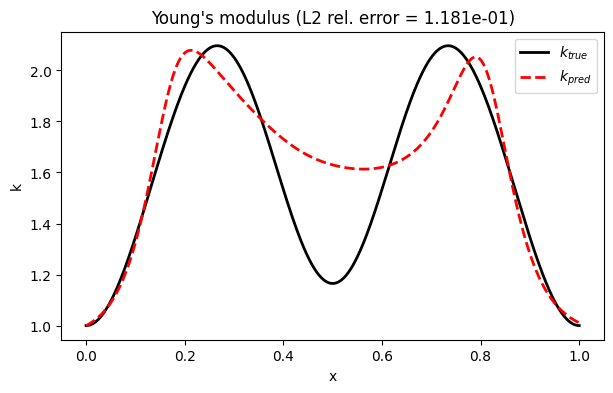
\includegraphics[width=\textwidth]{figures/ProblemA_Ktrue_Kpred.png} 
        \caption{$k_{pred}$ vs.\ $k_{true}$}
    \end{subfigure}
    %
    \begin{subfigure}[b]{0.48\textwidth}
        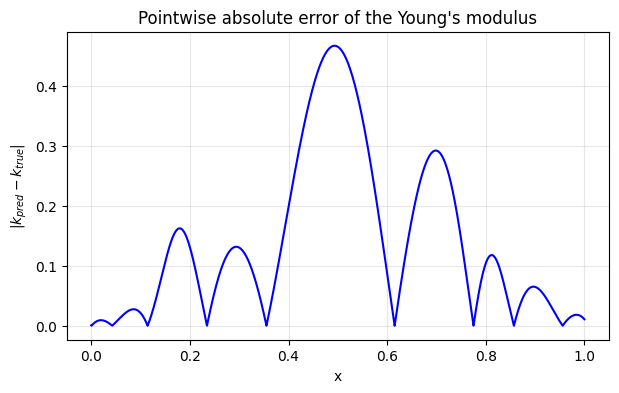
\includegraphics[width=\textwidth]{figures/ProblemA_abs_kpred-ktrue.png}
        \caption{$|k_{pred}-k_{true}|$}
    \end{subfigure}
    %
    \begin{subfigure}[b]{0.6\textwidth}
        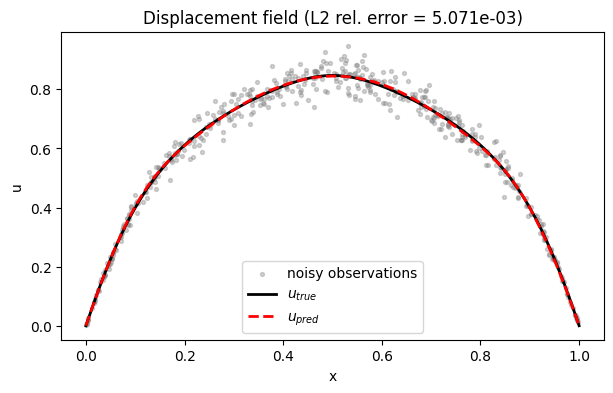
\includegraphics[width=\textwidth]{figures/ProblemA_upred_utrue.png} % TODO: u_pred vs u_true
        \caption{$u_{pred}$ vs.\ $u_{true}$}
    \end{subfigure}
    \caption{Problem A: recovered Young's modulus and displacement field.}
    \label{fig:problem_A_2}
\end{figure}


%%%%%%%%%%%%%%%%%%%%%%
\chapter{Problem B}
\label{ch:problem_B}
%
\section{Problem Description}
The pressure $u(x)$ in a two-phase porous medium on $\Omega = [0,1]^2$
satisfies the Darcy equation
\begin{equation}
    -\nabla\cdot\big(\mu(x)\,\nabla u\big) = 0, \qquad x \in \Omega,
    \label{eq:B_pde}
\end{equation}
where the permeability $\mu$ takes the value $10$ in the sandstone phase
and $2$ in the mudstone matrix; the phase geometry is given as a
$128\times128$ pixel image. Dirichlet data drive the flow from left to
right: $u = 1$ at $x_1 = 0$, $u = 0$ at $x_1 = 1$, and linear interpolation
on the top and bottom edges. Since all four boundary segments agree with
the single function $g(x) = 1 - x_1$, the boundary condition is simply
$u = 1 - x_1$ on $\partial\Omega$. The difficulty lies in the discontinuous
coefficient: the pressure gradient jumps across the phase interfaces.
%
\section{Methodology}
%
\subsubsection{The method selection}
We use the Deep Ritz method \cite{e2018deepritz}. Equation \eqref{eq:B_pde}
is symmetric elliptic, so its weak solution is the unique minimizer of the
energy
\begin{equation}
    E(u) = \int_\Omega \frac{\mu(x)}{2}\,|\nabla u(x)|^2 \, dx
    \label{eq:B_energy}
\end{equation}
over all fields satisfying the boundary condition. Two properties make this
formulation attractive for a discontinuous coefficient. Only first
derivatives of $u$ appear, and $\mu$ is merely evaluated but never
differentiated. A strong-form PINN, in contrast, would need
$\nabla\mu\cdot\nabla u$, and $\nabla\mu$ of a piecewise-constant field is
zero inside the phases and undefined on the interfaces, so the strong
residual is wrong exactly where the solution is difficult.

We initially implemented the weak-form ParticleWNN
\cite{zang2023particlewnn}, which also avoids differentiating $\mu$. It
performed noticeably worse in our tests: its loss consists of many local
integrals over small balls, each approximated by quadrature, and for balls
crossing the pixelated interfaces the quadrature error is large enough that
the optimizer can reduce the loss while the true error grows. The Deep Ritz
loss does not have this failure mode, because its Monte-Carlo estimator of
\eqref{eq:B_energy} is unbiased: in expectation, lowering the loss always
lowers the energy. In our runs Deep Ritz reached roughly half the error of
ParticleWNN at a fraction of the training cost, which settled the choice.
%
\subsubsection{The loss function}
The boundary condition is built into the ansatz,
\begin{equation}
    u_\theta(x) = (1 - x_1) + x_1(1-x_1)\,x_2(1-x_2)\,\mathcal{N}(x;\theta),
\end{equation}
so that $u_\theta = 1 - x_1$ holds exactly on all of $\partial\Omega$ and
the minimization is unconstrained -- no boundary penalty and no loss weight
at all. The loss is the Monte-Carlo energy
\begin{equation}
    \mathcal{L}(\theta) = \frac{1}{N}\sum_{i=1}^{N}
    \frac{\mu(x_i)}{2}\,\big|\nabla u_\theta(x_i)\big|^2 ,
\end{equation}
with $\nabla u_\theta$ from automatic differentiation and $\mu(x_i)$ from a
nearest-pixel lookup. Instead of uniform sampling we use stratified
sampling: one uniformly jittered point in each of the $128^2$ pixel cells
per epoch ($N = 16384$). Because $\mu$ is constant within a pixel, this
removes most of the variance of the energy estimate.
%
\subsubsection{The network structure}
The network (Table~\ref{tab:problem_B_net}) has $19761$ trainable
parameters.
%
\begin{table}[htbp]
\centering
\caption{Network architecture for Problem B.}
\label{tab:problem_B_net}
\begin{tabular}{llll}
\hline
\textbf{Layer} & \textbf{Size / Neurons} & \textbf{Activation} & \textbf{Notes} \\
\hline
Input          & 2   & --   & $(x_1,x_2)$, mapped to $[-1,1]^2$ \\
Hidden 1--4    & 80  & tanh & fully connected \\
Output         & 1   & --   & linear; then hard-BC transform \\
\hline
\end{tabular}
\end{table}
%
\subsubsection{The code link}
{https://github.com/omkulkarni01/PDE_Om_Anant_Kulkarni/blob/main/Problem_B.ipynb}
%
\section{Numerical Results}
%
\subsubsection{Experiment Setups}
%
\begin{table}[htbp]
\centering
\caption{Numerical setup for training (Problem B).}
\label{tab:problem_B_setup}
\begin{tabular}{ll}
\hline
\textbf{Parameter} & \textbf{Value} \\
\hline
Optimizer                  & Adam \\
Learning rate (initial)    & $1\times10^{-3}$ \\
Batch size                 & full batch (16384 stratified points per epoch) \\
Number of epochs           & 6000 \\
Learning rate scheduler    & StepLR, $\times 0.6$ every 1200 epochs \\
Loss weights               & none (single energy term, hard BCs) \\
Hardware                   & NVIDIA GeForce RTX 4050 Laptop GPU \\
Precision                  & Float32 \\
Random seed                & 1234 \\
\hline
\end{tabular}
\end{table}
%
Tricks: hard boundary constraint, stratified per-pixel sampling, input
normalization to $[-1,1]^2$, resampling at every epoch, and checkpointing
at the lowest training energy.
%
\subsubsection{Numerical Results}
Training took $42.8$~s. The final relative $L^2$ error on the
$128\times128$ reference grid is $3.21\times10^{-2}$, and the error curve
flattens after roughly $1000$ epochs. The remaining error is concentrated
along the phase interfaces: the exact pressure has a kink in its gradient
there, which a globally smooth tanh network can approximate but not
represent exactly. This is the known accuracy limit of smooth global ansatz
functions for interface problems and is visible as thin bands in the
pointwise error map.


%
\begin{figure}[ht]
    \centering
    \begin{subfigure}[b]{0.48\textwidth}
        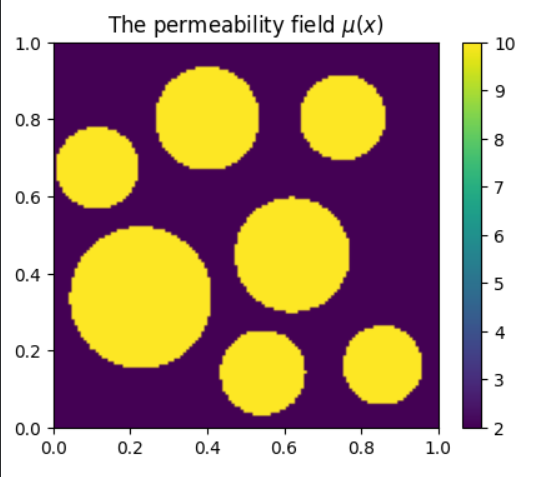
\includegraphics[width=\textwidth]{figures/PB_permeability.png}
        \caption{Permeability field and reference pressure $\mu(x)$.}
    \end{subfigure}

    \begin{subfigure}[b]{0.5\textwidth}
        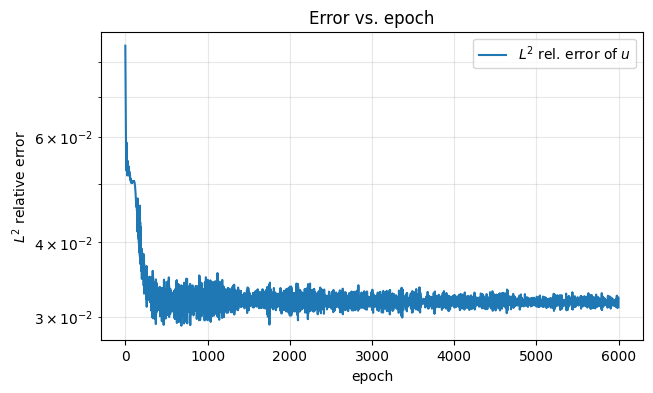
\includegraphics[width=\textwidth]{figures/PB_L2_epoch.png} % TODO: error-vs-epoch curve
        \caption{Relative $L^2$ error vs.\ epoch.}
    \end{subfigure}
    \caption{Problem B: input microstructure and training history.}
    \label{fig:problem_B_1}
\end{figure}
%
\paragraph{Interpretation and possible improvements.}
The result validates the reasoning behind the model choice: the Deep Ritz
energy only evaluates $\mu$ and only differentiates $u$ once, so the
discontinuous coefficient never enters a derivative, and training is stable
from the first epoch, unlike the ParticleWNN attempt, whose ball
quadrature interacted badly with the pixelated interfaces. At the same
time, the result exposes the method's intrinsic ceiling. Two facts locate
it precisely: the error curve flattens after about $1000$ of the $6000$
epochs, and wider networks in preliminary tests did not move the plateau,so neither optimization nor capacity is limiting. What limits accuracy is
representation: the exact pressure has a kinked gradient at every phase
interface, a $C^\infty$ tanh ansatz must round these kinks off, and the
$\sim 3\%$ error is the integrated cost of that rounding, visible as thin
bands along the interfaces in the error map. One small implementation
refinement is worth noting: the checkpoint is selected by the lowest
\emph{stochastic} energy estimate, which favours lucky sampling draws; the
final-epoch model was in fact marginally better ($3.11\times10^{-2}$), and
selecting by a running average of the energy would remove this artefact at
no cost. Substantial further gains, however, would require changing the
ansatz rather than the training. A phase-indicator input feature or a per-phase domain-decomposition network with interface conditions which
goes beyond the methods treated in the course and was not attempted within
the project time.

\begin{figure}[ht]
    \centering
    \begin{subfigure}[b]{0.48\textwidth}
        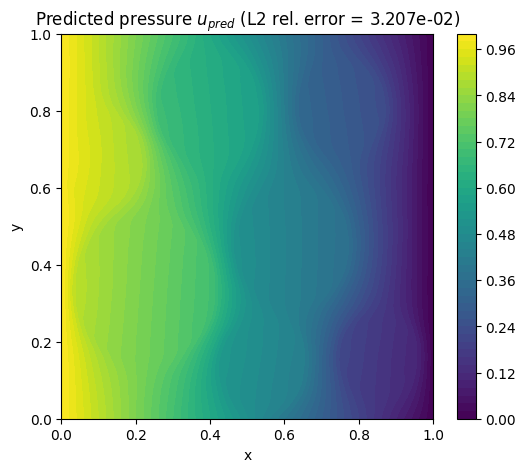
\includegraphics[width=\textwidth]{figures/PB_Predicted_pressure_L2.png} % TODO: u_pred
        \caption{Predicted $u_{pred}$}
    \end{subfigure}
    %
    \begin{subfigure}[b]{0.48\textwidth}
        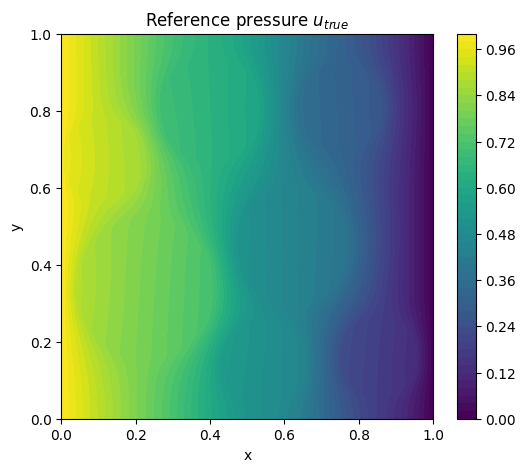
\includegraphics[width=\textwidth]{figures/PB_Utrue.png} % TODO: u_true
        \caption{Reference $u_{true}$}
    \end{subfigure}
    %
    \begin{subfigure}[b]{0.48\textwidth}
        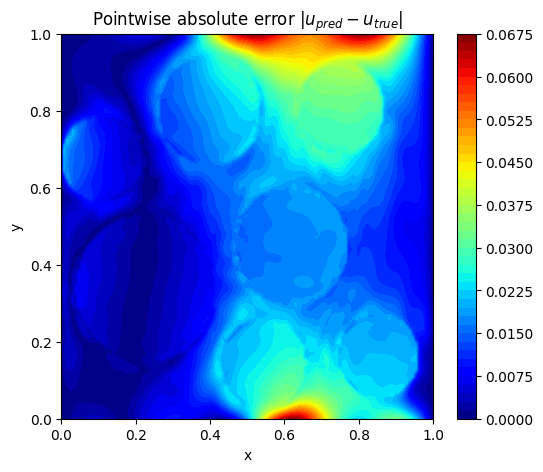
\includegraphics[width=\textwidth]{figures/PB_abs_upred-utrue.png} % TODO: |u_pred - u_true|
        \caption{$|u_{pred}-u_{true}|$}
    \end{subfigure}
    \caption{Problem B: predicted pressure, reference, and pointwise error.}
    \label{fig:problem_B_2}
\end{figure}

%%%%%%%%%%%%%%%%%%%%%%
\chapter{Problem C}
\label{ch:problem_C}
%
\section{Problem Description}
The temperature $u(x,y)$ in a heterogeneous solid on $\Omega = [0,1]^2$
solves
\begin{equation}
    -\nabla\cdot\big(a(x,y)\,\nabla u\big) = f \;\;\text{in } \Omega,
    \qquad u = 0 \;\;\text{on } \partial\Omega,
\end{equation}
with $f = 10$ and a spatially varying conductivity $a > 0$. The task is not
to solve one instance but to learn the solution operator $a \mapsto u$ from
$1000$ FEM-computed pairs $(a^{(j)}, u^{(j)})$ on a $128\times128$ grid, so
that the temperature field of a new microstructure can be predicted at
negligible cost. Accuracy is measured by the mean per-sample relative $L^2$
error over $200$ unseen test conductivities.
%
\section{Methodology}
%
\subsubsection{The method selection}
We use a Fourier Neural Operator (FNO) \cite{li2021fno}. The data is
aligned grid-to-grid, plentiful, and purely supervised as per the setting designed for FNO. Two properties of the underlying operator match the
FNO's inductive bias. The solution operator of an elliptic problem is
non-local (a local change of $a$ influences $u$ everywhere), and the FNO's
spectral convolutions give every layer a global receptive field, which a
CNN of comparable size does not have. The operator is also smoothing, so
its action is dominated by low Fourier modes, and the FNO's mode truncation
exploits exactly that. A DeepONet \cite{lu2021deeponet} could be applied
as well, but on aligned-grid Darcy-type benchmarks it is consistently less
accurate than the FNO, so the FNO is the natural choice when no unlabeled
data needs to be incorporated.

Since pre-built implementations are not allowed, all components are written
from scratch. In particular, no FFT routine is used: for the kept frequency
set $K = \{0,\dots,m-1\}\cup\{S-m,\dots,S-1\}$ we precompute the partial
DFT matrix $F_{kn} = e^{-2\pi i k n / S}$ directly from the definition and
apply the truncated two-dimensional transform as two matrix products,
$\widehat{v} = F v F^{\top}$. Because only $2m \ll S$ frequencies are ever
used, this costs $\mathcal{O}(2mS)$ per one-dimensional transform and loses
no accuracy compared to an FFT. The notebook verifies the matrices against
the direct DFT summation and the inverse round-trip identity. The learnable
complex mode weights are stored as separate real and imaginary parameter
tensors.
%
\subsubsection{The loss function}
Training minimizes the mean per-sample relative $L^2$ loss
\begin{equation}
    \mathcal{L}(\theta) = \frac{1}{B}\sum_{j=1}^{B}
    \frac{\|u_\theta(a^{(j)}) - u^{(j)}\|_2}{\|u^{(j)}\|_2},
\end{equation}
which has the same form as the required test metric and normalizes away
amplitude differences between samples. The input is the conductivity image,
normalized pointwise with training-set statistics, concatenated with the
two coordinate channels $(x,y)$.
%
\subsubsection{The network structure}
The model (Table~\ref{tab:problem_C_net}) has $4727297$ parameters, most of
them in the complex mode weights.
%
\begin{table}[htbp]
\centering
\caption{FNO architecture for Problem C ($S=128$, $m=12$ modes, width $32$).}
\label{tab:problem_C_net}
\begin{tabular}{llll}
\hline
\textbf{Layer} & \textbf{Size} & \textbf{Activation} & \textbf{Notes} \\
\hline
Lifting $P$         & $3 \to 32$   & --   & pointwise linear \\
Fourier layers 1--4 & width $32$   & GELU & spectral conv ($24{\times}24$ modes) $+$ $1{\times}1$ conv skip \\
Projection $Q_1$    & $32 \to 128$ & GELU & pointwise linear \\
Projection $Q_2$    & $128 \to 1$  & --   & pointwise linear \\
\hline
\end{tabular}
\end{table}
%
\subsubsection{The code link}
{https://github.com/omkulkarni01/PDE_Om_Anant_Kulkarni/blob/main/Problem_C.ipynb}
%
\section{Numerical Results}
%
\subsubsection{Experiment Setups}
%
\begin{table}[htbp]
\centering
\caption{Numerical setup for training (Problem C).}
\label{tab:problem_C_setup}
\begin{tabular}{ll}
\hline
\textbf{Parameter} & \textbf{Value} \\
\hline
Optimizer                  & Adam (weight decay $10^{-4}$) \\
Learning rate (initial)    & $1\times10^{-3}$ \\
Batch size                 & 20 \\
Number of epochs           & 200 \\
Learning rate scheduler    & StepLR, $\times 0.5$ every 50 epochs \\
Hardware                   & NVIDIA GeForce RTX 4050 Laptop GPU \\
Precision                  & Float32 \\
Random seed                & 1234 \\
\hline
\end{tabular}
\end{table}
%
Tricks: pointwise Gaussian normalization of the input (training statistics
only), coordinate channels, the relative-$L^2$ loss instead of plain MSE,
weight decay, and checkpointing at the lowest training loss.
%
\subsubsection{Numerical Results}
Training took $1198$~s (about $20$ minutes; $6$~s per epoch). The final
mean relative $L^2$ error over the $200$ test samples is
$7.25\times10^{-3}$, i.e.\ below one percent, while inference for a new
conductivity field takes on the order of milliseconds. The intended
replacement of a full FEM solve per microstructure in a screening workflow.
The training loss ($2.9\times10^{-3}$) is somewhat below the test error,
i.e.\ the model overfits mildly. Additonally, the weight decay and the learning-rate decay
keep the gap moderate. The largest pointwise errors appear near steep
conductivity gradients, where the truncated Fourier representation is least
efficient. The prediction is visually
indistinguishable from the FEM reference over the bulk of the domain.

%
\begin{figure}[ht]
    \centering
    \begin{subfigure}[b]{0.48\textwidth}
        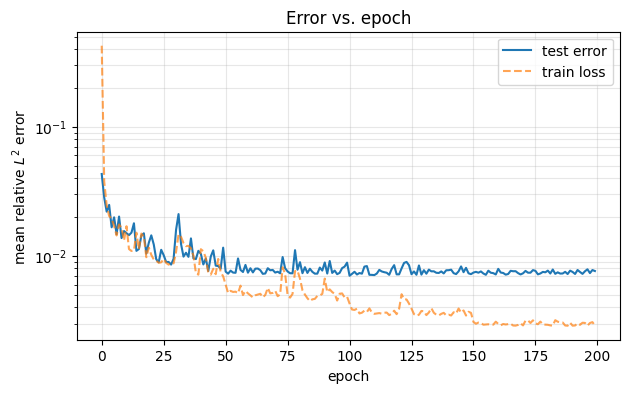
\includegraphics[width=\textwidth]{figures/PC_l2_epoch.png} % TODO: error-vs-epoch curve
        \caption{Mean relative $L^2$ error vs.\ epoch.}
    \end{subfigure}
    %
    \begin{subfigure}[b]{0.48\textwidth}
        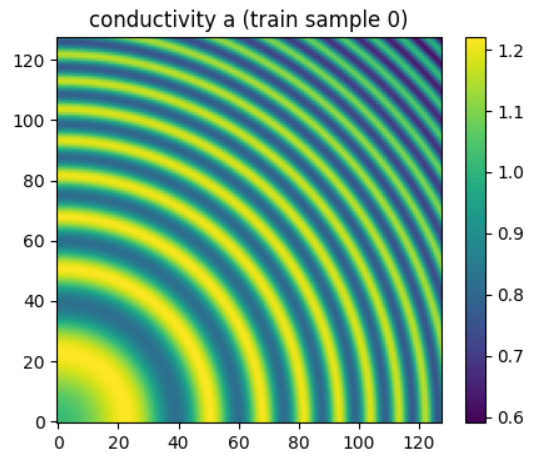
\includegraphics[width=\textwidth]{figures/PC_conductivity_inp.png} % TODO: input a (test instance 0)
        \caption{Input conductivity $a(x,y)$ (test instance 0).}
    \end{subfigure}
    %
        \begin{subfigure}[b]{0.48\textwidth}
        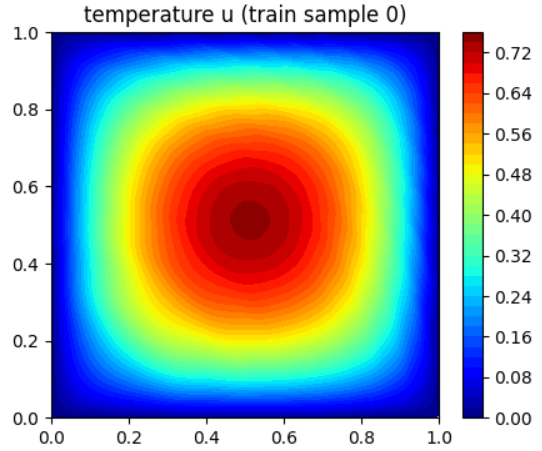
\includegraphics[width=\textwidth]{figures/PC_temp_inp.png} % TODO: input a (test instance 0)
        \caption{Temperature $a(x,y)$ (test instance 0).}
    \end{subfigure}
    \caption{Problem C: training history and input field of the first test instance.}
    \label{fig:problem_C_1}
\end{figure}

\paragraph{Interpretation and possible improvements.}
The error below one percent shows that the FNO is well suited to this
operator. The solution map of the elliptic problem is smooth and depends on
global information, and the spectral convolution layers capture this type of
mapping efficiently. This explains why the model achieves a level of accuracy
that the pointwise DeepONet approach does not reach on the aligned grid Darcy
benchmark.

The comparison between the training and test errors suggests that the model is
limited more by the amount of training data than by its capacity. The training
loss of $2.9\times10^{-3}$ is about $2.5$ times smaller than the test error,
which indicates that the network with $4.7$ million parameters starts to fit
the $1000$ training samples too closely. During the final training epochs the
test error varied between $7.2$ and $8.9\times10^{-3}$, and the learning rate
became small before the model reached a stable minimum.

Several straightforward changes could improve the results. These were not
included because of the available computing resources. Each training epoch
takes about $6$~s on a laptop GPU with $6$~GB of memory since the Fourier
transform is implemented with matrix multiplications instead of an FFT.
One possible improvement is data augmentation. The Darcy problem is unchanged
under the eight rotations and reflections of the grid, so applying the same
transformation to both $a$ and $u$ increases the effective training set by a
factor of eight without generating additional data. This could reduce the gap
between the training and test errors. Another option is to train for more
epochs while reducing the learning rate more gradually. For example, training
for $400$ epochs with the learning rate reduced every $100$ epochs could allow
the test error to converge more smoothly. Training several FNO models with
different random initializations and combining their predictions could also
improve the final accuracy, although this would require additional training
time.
%
\begin{figure}[ht]
    \centering
    \begin{subfigure}[b]{0.48\textwidth}
        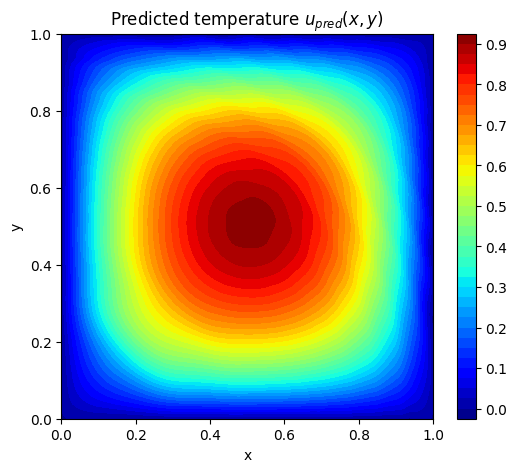
\includegraphics[width=\textwidth]{figures/PC_predicted_upred_temp.png} % TODO: u_pred
        \caption{Predicted $u_{pred}$}
    \end{subfigure}
    %
    \begin{subfigure}[b]{0.48\textwidth}
        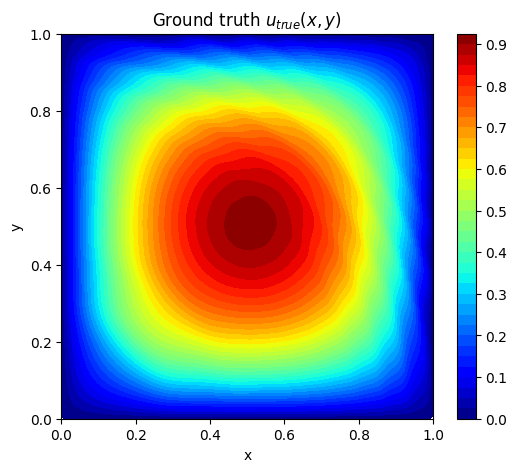
\includegraphics[width=\textwidth]{figures/PC_ground_truth_utrue.png} % TODO: u_true
        \caption{Ground truth $u_{true}$}
    \end{subfigure}
    %
    \begin{subfigure}[b]{0.48\textwidth}
        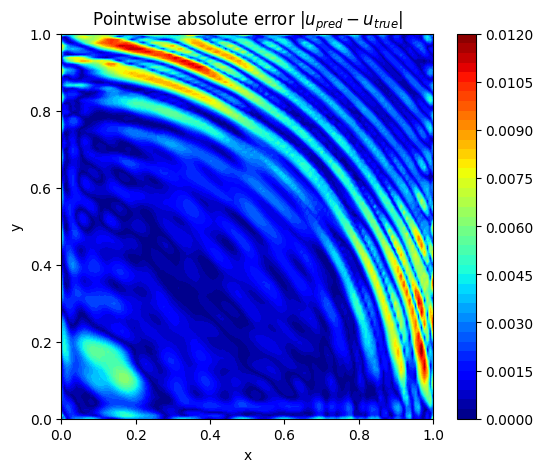
\includegraphics[width=\textwidth]{figures/PC_abs_ured-utrue.png} % TODO: |u_pred - u_true|
        \caption{$|u_{pred}-u_{true}|$}
    \end{subfigure}
    \caption{Problem C: prediction, reference, and pointwise error (test instance 0).}
    \label{fig:problem_C_2}
\end{figure}
\\

%%%%%%%%%%%%%%%%%%%%%%
\chapter{Problem D}
\label{ch:problem_D}
%
\section{Problem Description}
The vehicle velocity $u(x,t)$ on a road segment follows the viscous Burgers
equation
\begin{equation}
    u_t + u\,u_x = \nu\,u_{xx}, \qquad x \in (-1,1),\; t \in (0,1],
    \qquad u(\pm 1, t) = 0,
    \label{eq:D_pde}
\end{equation}
with $\nu = 0.1/\pi$ and initial profile $u(x,0) = a(x)$. The goal is again
an operator: $a \mapsto u(\cdot,\cdot)$. The twist is that the dataset is
only partially labeled $200$ initial conditions come with their FDM
solutions on a $200\times256$ space-time grid, while $1800$ further initial
conditions have no solution attached. A method that uses only the labeled
pairs discards $90\%$ of the available data.
%
\section{Methodology}
%
\subsubsection{The method selection}
We use a physics-informed DeepONet \cite{lu2021deeponet, wang2021pideeponet}.
The DeepONet represents the operator as
\begin{equation}
    u_\theta(a)(x,t) = (1 - x^2) \sum_{k=1}^{p} b_k(a)\,\tau_k(x,t) + b_0,
    \label{eq:D_deeponet}
\end{equation}
where the branch network $b$ encodes the initial field sampled at the $256$
sensors and the trunk network $\tau$ takes the continuous coordinates
$(x,t)$. This structure is what allows the unlabeled data to contribute:
because the output is differentiable in $(x,t)$ by automatic
differentiation, the Burgers residual of \eqref{eq:D_pde} and the initial
condition $u(x,0) = a(x)$ can be imposed on the $1800$ unlabeled samples as
physics losses. A Fourier Neural Operator would predict on a fixed grid and
would need finite differences for the residual, and a purely data-driven
operator network would simply ignore the unlabeled majority of the dataset.
The prefactor $(1-x^2)$ in \eqref{eq:D_deeponet} vanishes at $x = \pm1$, so
the homogeneous Dirichlet conditions hold exactly (the dataset initial
fields satisfy $a(\pm1) = 0$, so the initial condition is consistent with
this ansatz).

We train in two phases, a choice based on runtime measurements: an epoch
with the residual term costs far more than a purely supervised epoch
(second-order automatic differentiation on all collocation points), and
early in training the residual contributes little. Phase one therefore
minimizes only the data and initial-condition losses; phase two adds the
residual on the unlabeled samples with a reduced learning rate and pushes
the error well below the plateau of the supervised phase.
%
\subsubsection{The loss function}
With loss weights $w_{ic}$ and $w_{pde}$,
\begin{equation}
    \mathcal{L} =
    \underbrace{\overline{\big(u_\theta(a^{lab})(x_i,t_i) - u^{lab}_i\big)^2}}_{\text{data, labeled}}
    + w_{ic}\,\underbrace{\overline{\big(u_\theta(a^{unl})(x_s,0) - a^{unl}(x_s)\big)^2}}_{\text{IC, unlabeled}}
    + w_{pde}\,\underbrace{\overline{\big(u_t + u\,u_x - \nu\,u_{xx}\big)^2}}_{\text{residual, unlabeled}} ,
\end{equation}
with $w_{ic} = 5$ and $w_{pde} = 1$. Per epoch, the data term uses $100$
labeled samples at $2048$ randomly drawn space-time grid points (the
subsampling bounds memory and acts as augmentation); the physics terms use
$100$ unlabeled samples, the IC at all $256$ sensors, and the residual at
$400$ fresh random collocation points per sample. For the residual, the
branch output is repeated per collocation point so that a single backward
pass yields the derivatives $u_t$, $u_x$, $u_{xx}$ for every
(sample, point) pair.
%
\subsubsection{The network structure}
The model (Table~\ref{tab:problem_D_net}) has $125129$ trainable
parameters.
%
\begin{table}[htbp]
\centering
\caption{DeepONet architecture for Problem D (basis size $p = 100$).}
\label{tab:problem_D_net}
\begin{tabular}{llll}
\hline
\textbf{Network} & \textbf{Layers} & \textbf{Activation} & \textbf{Notes} \\
\hline
Branch  & $256 \to 128 \to 128 \to 128 \to 100$ & tanh & input: $a$ at 256 sensors \\
Trunk   & $2 \to 128 \to 128 \to 128 \to 100$   & tanh & input: $(x, 2t{-}1)$; output $\times (1-x^2)$ \\
Bias    & 1 scalar $b_0$                        & --   & trainable \\
\hline
\end{tabular}
\end{table}
%
\subsubsection{The code link}
{https://github.com/omkulkarni01/PDE_Om_Anant_Kulkarni/blob/main/Problem_D.ipynb}
%
\section{Numerical Results}
%
\subsubsection{Experiment Setups}
%
\begin{table}[htbp]
\centering
\caption{Numerical setup for training (Problem D).}
\label{tab:problem_D_setup}
\begin{tabular}{ll}
\hline
\textbf{Parameter} & \textbf{Value} \\
\hline
Optimizer                  & Adam \\
Learning rate              & $1\times10^{-3}$ (phase 1), $2\times10^{-4}$ (phase 2) \\
Batch size                 & 100 labeled $\times$ 2048 pts; 100 unlabeled $\times$ 400 colloc.\ pts \\
Number of epochs           & 30000 (phase 1) $+$ 10000 (phase 2) \\
Learning rate scheduler    & StepLR, $\times 0.5$ every 8000 / 3000 epochs \\
Loss weights               & $w_{data}=1$, $w_{ic}=5$, $w_{pde}=1$ \\
Hardware                   & NVIDIA GeForce RTX 4050 Laptop GPU \\
Precision                  & Float32 \\
Random seed                & 1234 \\
\hline
\end{tabular}
\end{table}
%
Tricks: the two-phase curriculum, the hard boundary factor $(1-x^2)$,
normalization of $t$ to $[-1,1]$ in the trunk input, fresh collocation and
grid-point subsets at every epoch, and per-phase checkpointing at the
lowest training loss.
%
\subsubsection{Numerical Results}
Training took $1298$~s in total (about $22$ minutes, most of it in the
physics phase). The purely supervised phase plateaued at a mean relative
$L^2$ error of $1.01\times10^{-1}$; adding the Burgers residual on the
unlabeled initial conditions in phase two reduced the error to
$4.08\times10^{-2}$ which is an improvement by a factor of about $2.5$. The residual term propagates each
unlabeled initial condition into the interior of the space-time domain, so
the operator is effectively trained on ten times more initial conditions
than the labeled set alone provides,this is
the expected semi-supervised effect. The largest pointwise errors occur
along the steep fronts that develop from the nonlinear convection term,
where the smooth basis expansion \eqref{eq:D_deeponet} is least efficient.
%
\begin{figure}[ht]
    \centering
    \begin{subfigure}[b]{0.48\textwidth}
        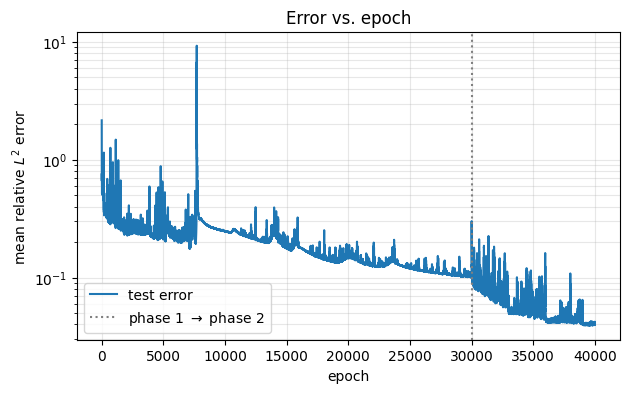
\includegraphics[width=\textwidth]{figures/PD_l2_epoch.png} % TODO: error-vs-epoch curve
        \caption{Mean relative $L^2$ error vs.\ epoch (phase boundary marked).}
    \end{subfigure}
    %
    \begin{subfigure}[b]{0.48\textwidth}
        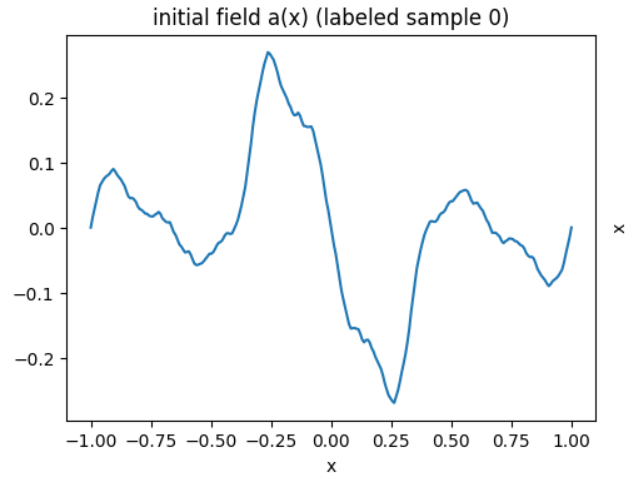
\includegraphics[width=\textwidth]{figures/PD_initial_ax.png} % TODO: initial condition a(x)
        \caption{Initial condition $a(x)$ (test instance 0).}
    \end{subfigure}
    \caption{Problem D: training history and first test initial condition.}
    \label{fig:problem_D_1}
\end{figure}
\paragraph{Interpretation and possible improvements.}
The improvement by a factor of $2.5$ during the physics informed stage is the
main result of this experiment. It demonstrates the advantage of using an
operator network with a continuous coordinate trunk, since this architecture
can use unlabeled initial conditions as additional training data through
automatic differentiation. In this case, the information provided by the
physics residual was more valuable than simply increasing the amount of labeled
data. After supervised training with $200$ labeled samples, the test error
stabilized at $10.1\%$. Including the physics residual from the $1800$
unlabeled samples reduced the error to $4.1\%$. The training history suggests that the current result is not the best
performance the model could achieve. At the end of the second training stage,
the test error was still decreasing, falling from $5.4\%$ at epoch $8000$ to
$4.0\%$ at epoch $10000$. This indicates that training ended before the model
had fully converged. Each epoch in the physics informed stage requires second
order automatic differentiation over $40000$ sample and point pairs, which
limited the total training time on the available laptop GPU. Extending this
stage of training would therefore be the most effective way to improve the
results.

The residual loss, which remained close to $10^{-3}$, also suggests that the
model had not yet reached its capacity. Increasing the basis size beyond
$p=100$ and using more collocation points for each sample could allow the
optimization to continue improving. Further gains may also come from sampling
collocation points more densely in regions where the solution changes rapidly,
especially near the sharp convective fronts. Replacing the fixed loss weights
$w_{ic}=5$ and $w_{pde}=1$ with adaptive weighting during training could also
provide a better balance between the initial condition and the physics
constraints.
%
\begin{figure}[ht]
    \centering
    \begin{subfigure}[b]{0.6\textwidth}
        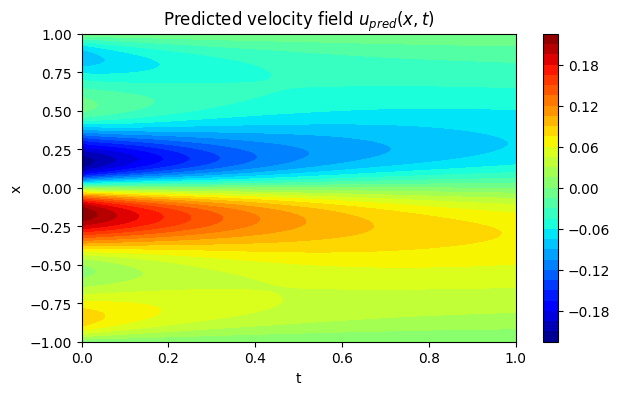
\includegraphics[width=\textwidth]{figures/PD_upred.png} % TODO: u_pred
        \caption{Predicted $u_{pred}(x,t)$}
    \end{subfigure}
    %
    \begin{subfigure}[b]{0.6\textwidth}
        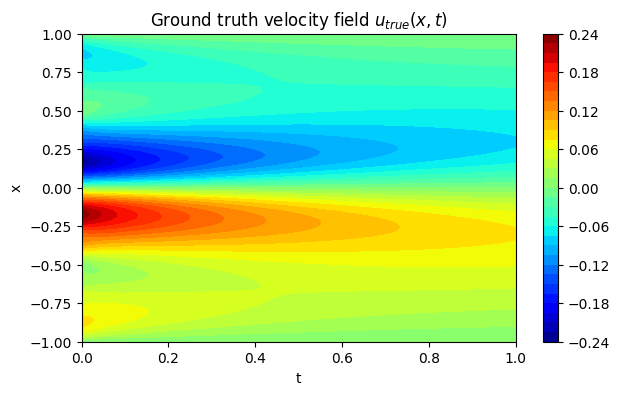
\includegraphics[width=\textwidth]{figures/PD_utrue.png} % TODO: u_true
        \caption{Ground truth $u_{true}(x,t)$}
    \end{subfigure}
    %
    \begin{subfigure}[b]{0.6\textwidth}
        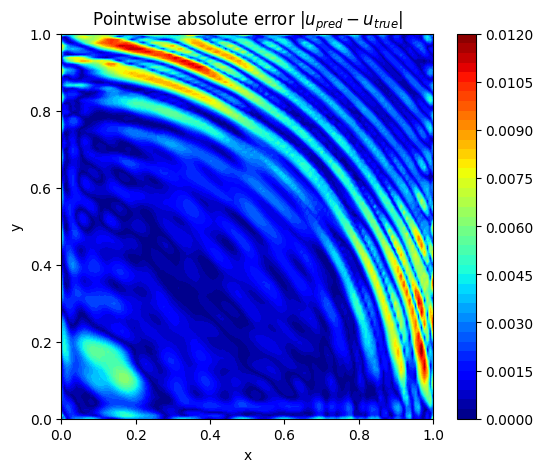
\includegraphics[width=\textwidth]{figures/PC_abs_ured-utrue.png} % TODO: |u_pred - u_true|
        \caption{$|u_{pred}-u_{true}|$}
    \end{subfigure}
    \caption{Problem D: predicted velocity field, reference, and pointwise error (test instance 0).}
    \label{fig:problem_D_2}
\end{figure}
